\section{Getting started}
\genHeader 

Here's how we've organized our handbooks; Black, red, and blue headers are used to separate common, visual, and textual syntax instructions
(Fig~\ref{pageExamples}).

\begin{figure}[htbp] \centering
  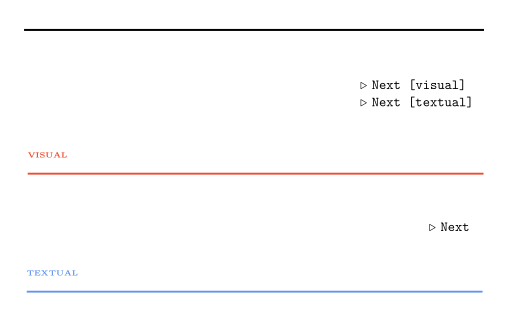
\includegraphics[width=0.9\textwidth]{headers}
	\caption{Page headers and links}
	\label{pageExamples}
\end{figure}

You'll find a \mbox{ $\triangleright$ {\texttt{link}} } at the bottom of some pages. These will take you to the next appropriate place for your syntax. You are
still welcome to go through the entire handbook page by page. In fact, we encourage it and hope you'll compare the differences and similarities between the two
specifications. But be warned! If what you're doing isn't matching what you see, you may be reading the wrong instructions.

If, however, you're finding that the screenshots we've taken aren't matching your screen and you ARE in the right place, please send us an email at
\href{mailto:contact@moflon.org}{contact@moflon.org} and let us know. They get outdated so fast! They just grow up, move on, start doing their own thing and
\ldots uh, wait a second. We're talking about pictures here.

Here are some guidelines to help you decide which syntax to use:

\begin{itemize}

\item[$\blacktriangleright$] If you have used a UML tool before and feel comfortable with the standard UML diagrams, then you might prefer our visual syntax.

\item[$\blacktriangleright$] If you do not like switching tools, and want everything integrated completely in Eclipse with zero installation, then you should
stick to our textual syntax.

\item[$\blacktriangleright$] If you use a Mac (or some other *Nix system) then you will need virtualisation software to run Windows and install the required
UML tool for our visual syntax. Most maconians find this insulting and of course choose our textual syntax.

\item[$\blacktriangleright$] As a final remark, consider that graph transformations obviously have something to do with graphs, which are inherently two
dimensional structures. A visual syntax thus has some obvious advantages and is what we (currently) prefer and use internally (eMoflon is built with eMoflon).

\end{itemize}
